\chapter{Sistema di autenticazione}


\section{Scopo del sistema}

Il sistema di autenticazione ha lo scopo di gestire le richieste di autenticazione da parte degli utenti e di fornire un token di sessione valido per l'accesso alle risorse protette.

\section{Descrizione del sistema}

Il sistema di autenticazione è definito da un microservizio che espone un'interfaccia REST per la gestione delle richieste di autenticazione degli utenti. Il microservizio è inoltre responsabile della generazione e della validazione dei token di sessione.

I token di sessione utilizzati sono del tipo JWT (JSON Web Token) e sono composti da tre parti separate da un punto. La prima parte contiene le informazioni relative all'algoritmo di hashing utilizzato per la firma del token, la seconda parte contiene le informazioni relative all'utente autenticato e la terza parte contiene la firma del token.

\section{Architettura del sistema}

Il sistema utilizza un'architettura esagonale, in cui il core del sistema si occupa della business logic ed offre:
\begin{itemize}
    \item Generazione dei JWT;
    \item Refresh dei JWT;
    \item Autenticazione degli utenti.
\end{itemize}

\begin{figure}[H]
    \centering
    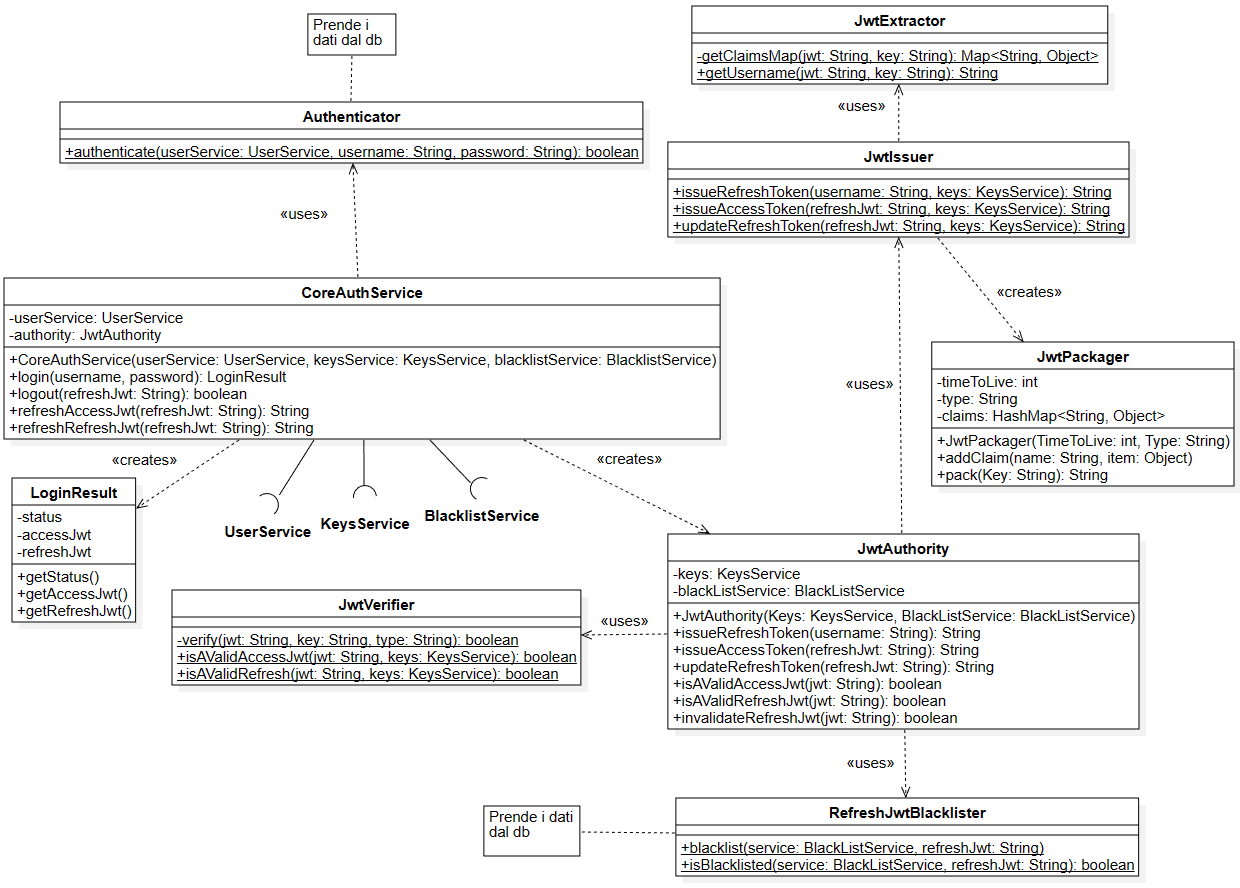
\includegraphics[width=\textwidth]{img/classi_auth.png}
    \caption{Diagramma delle classi del sistema di autenticazione}
\end{figure}

Il sistema offre poi un'interfaccia di tipo REST, e si connette sempre tramite l'utilizzo del sistema a porte ad un Database per la memorizzazione dei dati.

\subsection{Il core del sistema}

\subsubsection{Le classi base dell'architettura esagonale}

Nell'architettura esagonale, il core del sistema è composto da tre classi base: il port, l'adapter e il modello.

%%Qui vanno definite le responsabilità di ogni classe.
\begin{itemize}
    \item \textbf{Authenticator:} si occupa dell'autenticazione dell'utente, verificando che l'username e la password fornite siano corrette.
    \item \textbf{Blacklister:} si occupa di inserire in una \textit{blacklist} i jwt di refresh che si vogliono rendere inutilizzabili.
    \item \textbf{JwtExtractor:} si occupa di estrarre la mappa chiave-valore dal jwt. In particolare nel nostro caso serve estrarre l'username dell'utente.
    \item \textbf{JwtIssuer:} si occupa della creazione e della rigenerazione dei jwt (access o refresh), inserendo al loro interno l'username dell'utente.
    \item \textbf{JwtPackager:} si occupa della creazione e della firma di un generico jwt. Ha un tipo, una mappa chiave-valore e una scadenza.
    \item \textbf{JwtVerifier:} si occupa di verificare che un jwt ricevuto sia valido, ovvero che abbia un determinato tipo (access o refresh), non sia ancora scaduto e che abbia la mappa chiave-valore.
\end{itemize}


\subsection{I JWT}

Il sistema generale è pensato per utilizzare due tipologie di Token. Viene utilizzato un token di autorizzazione, che viene utilizzato per l'autenticazione e per l'accesso alle risorse protette degli altri microservizi e un token di refresh, che viene utilizzato per la generazione di un nuovo token di autorizzazione.

Ognuno dei microservizi del sistema accetta come valido un token generato da questo microservizio. Non accetterà però come valido un token di refresh.

Il token di refresh viene infatti riconosciuto solamente da questo sistema.

Il token di refresh ha durata di 2h, mentre il token di autorizzazione ha durata di 10 minuti.

\section{Port Interfaccia REST}

L'interfaccia rest viene esposta all'esterno e permette di effettuare le operazioni discusse nelle sotto-sezioni successive.

\begin{itemize}
    \item POST /login
    \item POST /logout
    \item POST /refresh/refreshtoken
    \item POST /refresh/accesstoken
\end{itemize}

\subsection{POST /login}

Login permette di effettuare il login di un utente. L'utente deve fornire le credenziali di accesso, e il sistema risponderà con un token di autorizzazione e un token di refresh.

Le credenziali vengono fornite sotto formato JSON nel body della richiesta, e devono essere composte da username e password.

\subsection{POST /logout}

Logout permette di effettuare il logout di un utente. L'utente deve fornire il token di refresh, e il sistema risponderà con un messaggio di conferma.

Il sistema invalida il token di refresh fornito, e l'utente non potrà più utilizzarlo per generare nuovi token di autorizzazione.

Per invalidarlo, il sistema lo inserisce in una blacklist, e non lo accetterà più come valido.

Quando il token di refresh scade, il sistema lo rimuove dalla blacklist.

\subsection{POST /refresh/refreshtoken}

Refresh refreshtoken permette di generare un nuovo token di refresh. L'utente deve fornire il token di refresh, e il sistema risponderà con un nuovo token di refresh.

\subsection{POST /refresh/accesstoken}

Refresh accesstoken permette di generare un nuovo token di autorizzazione. L'utente deve fornire il token di refresh, e il sistema risponderà con un nuovo token di autorizzazione.

\section{Port Database}

Il sistema utilizza un database per memorizzare i JWT di accesso in blackilist.

Si immagina inoltre che il sistema utilizzi un database per memorizzare le credenziali degli utenti. Nella nostra versione attuale esistono però solamente due utenti e questi sono definiti all'interno del codice.

%%Qui va inserita la progettazione del db con progettazione concettuale(chiaramente molto ridotta).

%Va inoltre analizzato quale è il db migliore per gestire la coda fifo della blacklist. probabilmente un db non relazionale è più adatto. come mongoDB.
